\documentclass[12pt, a4paper, oneside, openright]{book}
%\documentclass[12pt,a4paper,english]{article}
\usepackage[english]{babel}
\usepackage[utf8]{inputenc}
\usepackage[T1]{fontenc}
\usepackage{microtype}
\usepackage[dvips]{graphicx}
\usepackage{xcolor}
\usepackage{times}
\usepackage{pdfpages}
\usepackage{appendix}
\usepackage{titlesec}
\usepackage{lscape}
\usepackage{amsmath}
\usepackage{amsthm}
\usepackage{amssymb}
\usepackage{amsfonts}
\usepackage{braket}
\usepackage[
breaklinks=true,colorlinks=true,
linkcolor=blue,urlcolor=blue,citecolor=blue,% PDF VIEW
%linkcolor=black,urlcolor=black,citecolor=black,% PRINT
bookmarks=true,bookmarksopenlevel=2]{hyperref}
\usepackage{geometry}
% PDF VIEW

%\usepackage[notocbib]{naturemag}
%\graphicspath{ {./images/} }
%\usepackage[
 % breaklinks=true,colorlinks=true,
  %linkcolor=blue,urlcolor=blue,citecolor=blue, PDF VIEW
  %linkcolor=black,urlcolor=black,citecolor=black, PRINT
  %bookmarks=true,bookmarksopenlevel=2]%{hyperref}
%\OnehalfSpacing
\linespread{1.0}
% %%% CHAPTER'S STYLE
% \chapterstyle{bianchi}
% % \chapterstyle{ger}
% % \chapterstyle{madsen}
% % \chapterstyle{ell}
%%% STYLE OF SECTIONS, SUBSECTIONS, AND SUBSUBSECTIONS
%\setsecheadstyle{\large\bfseries\sffamily\raggedright}
%\setsubsecheadstyle{\large\bfseries\sffamily\raggedright}
%\setsubsubsecheadstyle{\bfseries\sffamily\raggedright}
%\pagestyle{plain}
 %\renewcommand{\chaptermark}[1]{\markboth{{\sffamily\thechapter\ #1}}{}}
 %\makepagestyle{plain}
 %\makeevenfoot{plain}{\thepage}{}{}
 %\makeoddfoot{plain}{}{}{\thepage}
 %\makeevenhead{plain}{}{\leftmark}{}
 %\makeoddhead{plain}{}{\leftmark}{}
%\maxsecnumdepth{subsection} % chapters, sections, and subsections are %numbered
%\maxtocdepth{subsection} % chapters, sections, and subsections are in the %Table of Contents
\makeatletter
\newcommand\footnoteref[1]{\protected@xdef\@thefnmark{\ref{#1}}\@footnotemark}
\makeatother

\usepackage{graphicx}
\usepackage{caption}
\usepackage{subcaption}
\usepackage{mhchem}
\usepackage{fullpage}
\usepackage{xspace}
\usepackage{epigraph}
\usepackage{listings}
\usepackage{tikz}
\usepackage{framed}
\usepackage{calc}
\usepackage{fancyhdr, fancyvrb}
\pagestyle{fancy}
\usepackage{tcolorbox}
\usepackage{appendix}
\usepackage{makecell}
\usepackage{float}
\usepackage{multirow}


\usepackage[left=2.5cm, right=2.5cm, top=2.5cm,includefoot, bottom=2.5cm,showframe]{geometry}
\renewcommand{\headrulewidth}{1pt}
\fancyhead[L,RO]{\textbf{\thepage}}
\fancyhead[LO]{\textbf{\rightmark}}
%\fancyhead[RE]{\textbf{\leftmark}}
\fancyfoot[C,CO]{\empty}

\newcommand{\mytextformat}{\itshape\epigraphsize}
\newenvironment{mytext}{\mytextformat}{}
\newenvironment{mysource}{\scshape\hfill}{}
\renewcommand{\textflush}{mytext} 
\renewcommand{\sourceflush}{mysource}
\usepackage{xspace}
\usepackage[paper=portrait,pagesize]{typearea}




\begin{comment}
\fancyhead[LE,RO]{\textbf{\thepage}}
\fancyhead[LO]{\textbf{\rightmark}}
\fancyhead[RE]{\textbf{\leftmark}}
\fancyfoot[CE,CO]{\empty}
\end{comment}

\usepackage{multicol}
\usepackage{hyperref}
\hypersetup{colorlinks,linkcolor={blue},citecolor={red},urlcolor={cyan}}
\usepackage[backend=biber,style=numeric,citestyle=nature]



\lstset{language=Python}

%New colors defined below
\definecolor{codegreen}{rgb}{0.5,0.6,0}
\definecolor{codegray}{rgb}{0.5,0.5,0.5}
\definecolor{codepurple}{rgb}{0.58,0,0.82}
\definecolor{backcolour}{rgb}{0.95,0.95,0.92}
\renewcommand{\lstlistingname}{Code}% Listing -> Algorithm
\lstdefinestyle{mystyle}{
  backgroundcolor=\color{backcolour},   commentstyle=\color{codegreen},
  keywordstyle=\color{magenta},
  numberstyle=\tiny\color{codegray},
  stringstyle=\color{codepurple},
  basicstyle=\ttfamily\footnotesize,
  breakatwhitespace=false,         
  breaklines=true,                 
  captionpos=b,                    
  keepspaces=true,                 
  numbers=left,                    
  numbersep=5pt,                  
  showspaces=false,                
  showstringspaces=false,
  showtabs=false,                  
  tabsize=2}
%"mystyle" code listing set
\lstset{style=mystyle}




\lstset{style=mystyle}



\usepackage{xcolor}
\newcommand{\quotebox}[1]{\begin{center}\fcolorbox{white}{blue!15!gray!15}{\begin{minipage}{0.9\linewidth}\vspace{10pt}\center\begin{minipage}{0.8\linewidth}{\space\Huge``}{#1}{\hspace{1.5em}\break\null\Huge\hfill''}\end{minipage}\smallbreak\end{minipage}}\end{center}}





\usepackage{listings}
\usepackage{xcolor}

\definecolor{codegreen}{rgb}{0,0.6,0}
\definecolor{codegray}{rgb}{0.5,0.5,0.5}
\definecolor{codepurple}{rgb}{0.58,0,0.82}
\definecolor{backcolour}{rgb}{0.95,0.95,0.92}

\lstdefinestyle{mystyle}{
    backgroundcolor=\color{backcolour},   
    commentstyle=\color{codegreen},
    keywordstyle=\color{magenta},
    numberstyle=\tiny\color{codegray},
    stringstyle=\color{codepurple},
    basicstyle=\ttfamily\footnotesize,
    breakatwhitespace=false,         
    breaklines=true,                 
    captionpos=b,                    
    keepspaces=true,                 
    numbers=left,                    
    numbersep=5pt,                  
    showspaces=false,                
    showstringspaces=false,
    showtabs=false,                  
    tabsize=2
}
\begin{document}
%%%%%%%%%%%%%%%%%%%%%%%%%%%%%%%%%%%%%%%%%%%%%%%%%%%%%%%%%%%%%%%%%%%%%%%%
%%%%%%%%%%%%%%%%%%%%%%%%%%%%%%%%%%%%%%%%%%%%%%%%%%%%%%%%%%%%%%%%%%%%%%%%

%%%% TITLE PAGE
\begin{titlepage}
\begin{center}
\textbf{\LARGE OsloMet- Oslo Metropolitan University}\\[0.5cm] 
\textbf{\Large Department of Computer Science}\\[0.2cm]
\textbf{\Large Oslo Norway }\\[0.8cm]
\textbf{\Large ACIT4630-1 24V Advanced Machine Learning and Deep Learning}\\[0.2cm]
\vspace{20pt}


\begin{center}
\textbf{May 2024}\\
\end{center}
\vspace{20pt}

\par
\vspace{20pt}
\textbf{\Large \textcolor{blue}{Optimizing Mushroom Classification: Leveraging Transfer Learning with EfficientNetB0 Architecture}}\\
\vspace{25pt}
\vspace{1pt}
\textbf{{ Candidate number 107, 108 , 119 }}\\[0.1cm]
\vspace{25pt}


\end{center}

\par
\vfill
\end{titlepage}


%%% TABLE OF CONTENTS
\newpage
\tableofcontents
%  %End Sumário
//Viktoria
//Viktoria
\section{Methodology}

Our journey to develop a robust mushroom classification system began with a comprehensive search for a dataset that would serve as the foundation of our machine learning project. We conducted extensive research, leveraging academic repositories, online datasets, and domain-specific forums to identify a suitable corpus of mushroom images. This process involved a meticulous examination of each dataset's composition, quality, and relevance to our research objectives. 

After thorough deliberation and consultation with domain experts, we settled on a dataset comprising approximately 100,000 images sourced from diverse sources such as online repositories, scientific publications, and citizen science initiatives. On closer examination, however, we encountered several challenges inherent in the selected data set. Among these challenges, was the presence of multiple classes, which include poisonous, edible, conditionally edible, and deadly mushrooms, which complicated the classification task.

Furthermore, the dataset suffered from significant class imbalance, with the 'conditionally edible' class disproportionately represented, posing a potential bias in model training.

To mitigate these issues and streamline our research focus, we made the strategic decision to narrow our scope to the binary classification of mushrooms as either 'poisonous' or 'edible'. This decision not only aligned with the primary objectives of our study but also facilitated a more balanced and focused analysis. With the dataset curated and class imbalance addressed through careful selection, our attention turned to preprocessing the images to uniformity and compatibility with our chosen machine learning model. 

The dataset contains different species of poisonous and non poisonous class. There were numerous challanges like varying pattern, color, shape, background. Many of them looks anything else but not mushroom.


\begin{figure*}[!ht]
    \centering
    \begin{subfigure}{0.23\textwidth} % Adjust the width as needed
        \centering
        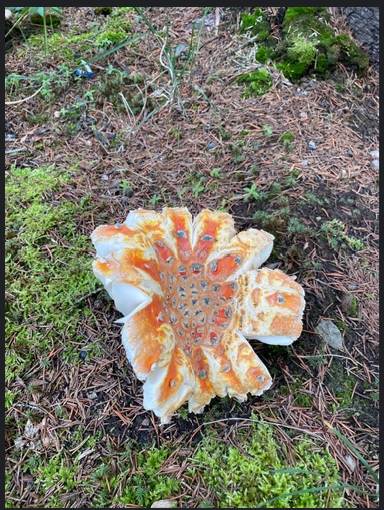
\includegraphics[height=3cm, width=\linewidth]{images/mushroom1.png}
        \caption{Mushroom 1} % Add caption for the first figure
    \end{subfigure}
    \hfill
    \begin{subfigure}{0.23\textwidth} % Adjust the width as needed
        \centering
        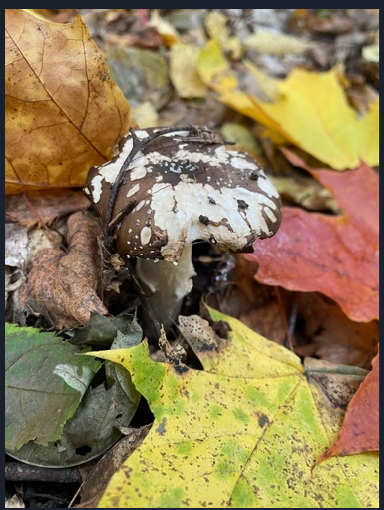
\includegraphics[height=3cm, width=\linewidth]{images/mushroom2.png}
        \caption{Mushroom 2} % Add caption for the second figure
    \end{subfigure}
    \hfill
    \begin{subfigure}{0.23\textwidth} % Adjust the width as needed
        \centering
        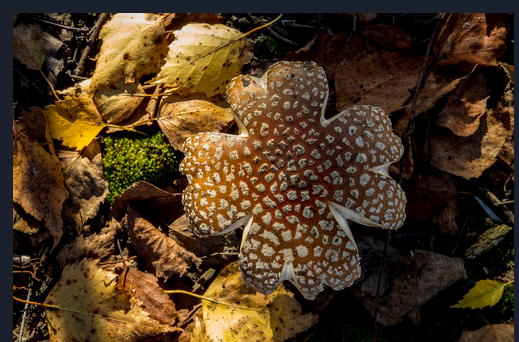
\includegraphics[height=3cm, width=\linewidth]{images/mushroom3.png}
        \caption{Mushroom 3} % Add caption for the third figure
    \end{subfigure}
    \hfill
    \begin{subfigure}{0.23\textwidth} % Adjust the width as needed
        \centering
        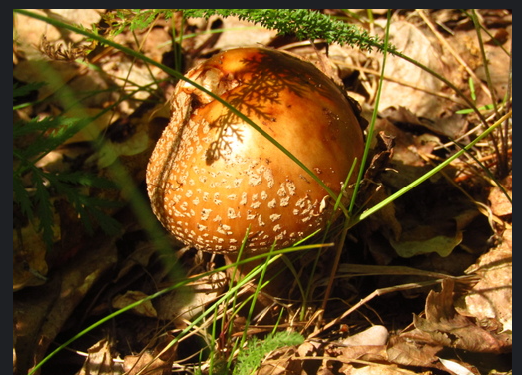
\includegraphics[height=3cm, width=\linewidth]{images/mushroom4.png}
        \caption{Mushroom 4} % Add caption for the fourth figure
    \end{subfigure}
    
    \vspace{0.5cm} % Adjust vertical space between rows
    
    \begin{subfigure}{0.23\textwidth} % Adjust the width as needed
        \centering
        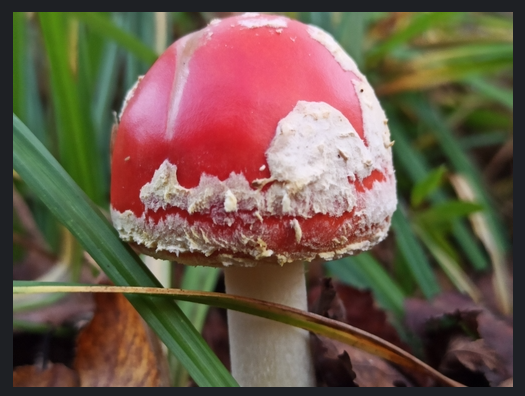
\includegraphics[height=3cm, width=\linewidth]{images/mushroom5.png}
        \caption{Mushroom 5} % Add caption for the first figure in the second row
    \end{subfigure}
    \hfill
    \begin{subfigure}{0.23\textwidth} % Adjust the width as needed
        \centering
        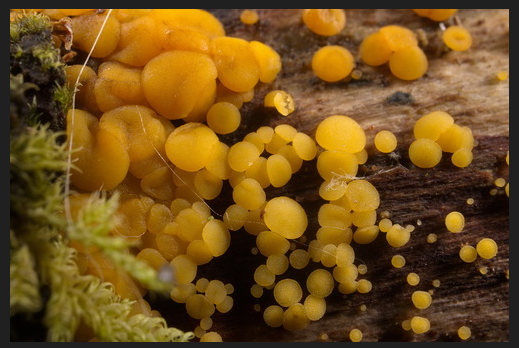
\includegraphics[height=3cm, width=\linewidth]{images/mushroom6.png}
        \caption{Mushroom 6} % Add caption for the second figure in the second row
    \end{subfigure}
    \hfill
    \begin{subfigure}{0.23\textwidth} % Adjust the width as needed
        \centering
        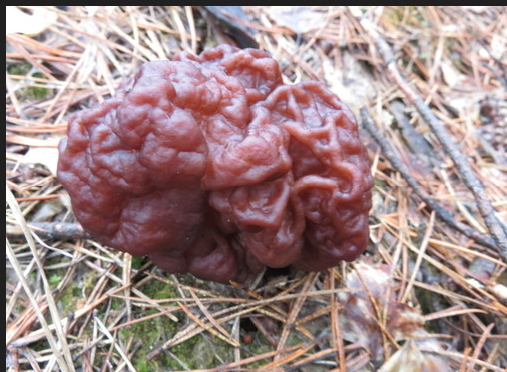
\includegraphics[height=3cm, width=\linewidth]{images/mushroom7.png}
        \caption{Mushroom 7} % Add caption for the third figure in the second row
    \end{subfigure}
    \hfill
    \begin{subfigure}{0.23\textwidth} % Adjust the width as needed
        \centering
        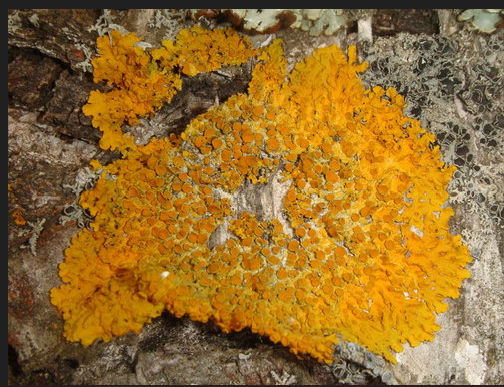
\includegraphics[height=3cm, width=\linewidth]{images/mushroom8.png}
        \caption{Mushroom 8} % Add caption for the fourth figure in the second row
    \end{subfigure}
    
    \caption{Different kinds of poisonous mushrooms} % Add a general caption for all figures
\end{figure*}




The initial inspection revealed inconsistencies in image sizes, necessitating resizing to a standardized format of 224x224 pixels. Additionally, we identified discrepancies in image formats, with some images in JPEG, JPG, and PNG formats. Of particular concern was the presence of PNG images, which introduced an additional alpha channel representing transparency, thereby deviating from the RGB color space used by the majority of the dataset. To rectify this discrepancy and ensure consistency in input data, we systematically converted all PNG images to the JPEG format, thus harmonizing the color channels across the entire dataset. Moreover, during the preprocessing stage, we encountered a subset of images that were corrupted or of insufficient quality for meaningful analysis. To maintain data integrity and prevent noise from influencing model performance, these corrupted images were systematically identified and removed from the dataset. This meticulous approach to data preprocessing was essential to ensure the reliability and robustness of our machine learning pipeline.

After carefully preparing the dataset, our next crucial step was model selection and architecture design. Recognizing the importance of utilizing state-of-the-art techniques for image classification, we conducted a comprehensive survey of modern models and architectures. While we first assessed the ResNet model, which has shown success in various image classification tasks, our preliminary experiments revealed suboptimal performance on our mushroom classification task. In response, we shifted our focus to EfficientNetB0, a recent and highly efficient convolutional neural network (CNN) architecture known for its superior performance on image classification.


With the EfficientNetB0 architecture selected as our backbone, we proceeded to fine-tune the model using transfer learning—a technique that leverages pre-trained models on large-scale datasets to accelerate learning on domain-specific tasks with limited labeled data. By transferring knowledge from the pre-trained EfficientNetB0 model, which was trained on ImageNet—a vast dataset comprising millions of labeled images spanning thousands of classes—we aimed to expedite the training process and enhance the model's ability to generalize across diverse mushroom images.

\section{Proposed architecture}
Our mushroom classification model utilizes the EfficientNetB0 architecture, renowned for its efficiency and performance in image classification tasks. Fine-tuning the pre-trained EfficientNetB0 model on our dataset allows it to adapt its parameters to the specific task of mushroom classification while leveraging knowledge learned from large-scale image datasets.
EfficientNetB0 is a unique convolutional neural network architecture because it prioritizes computational efficiency above performance to get cutting-edge results. To achieve that state of the art result, it proposes a few new ideas:
\begin{figure}[!ht]
    \centering
    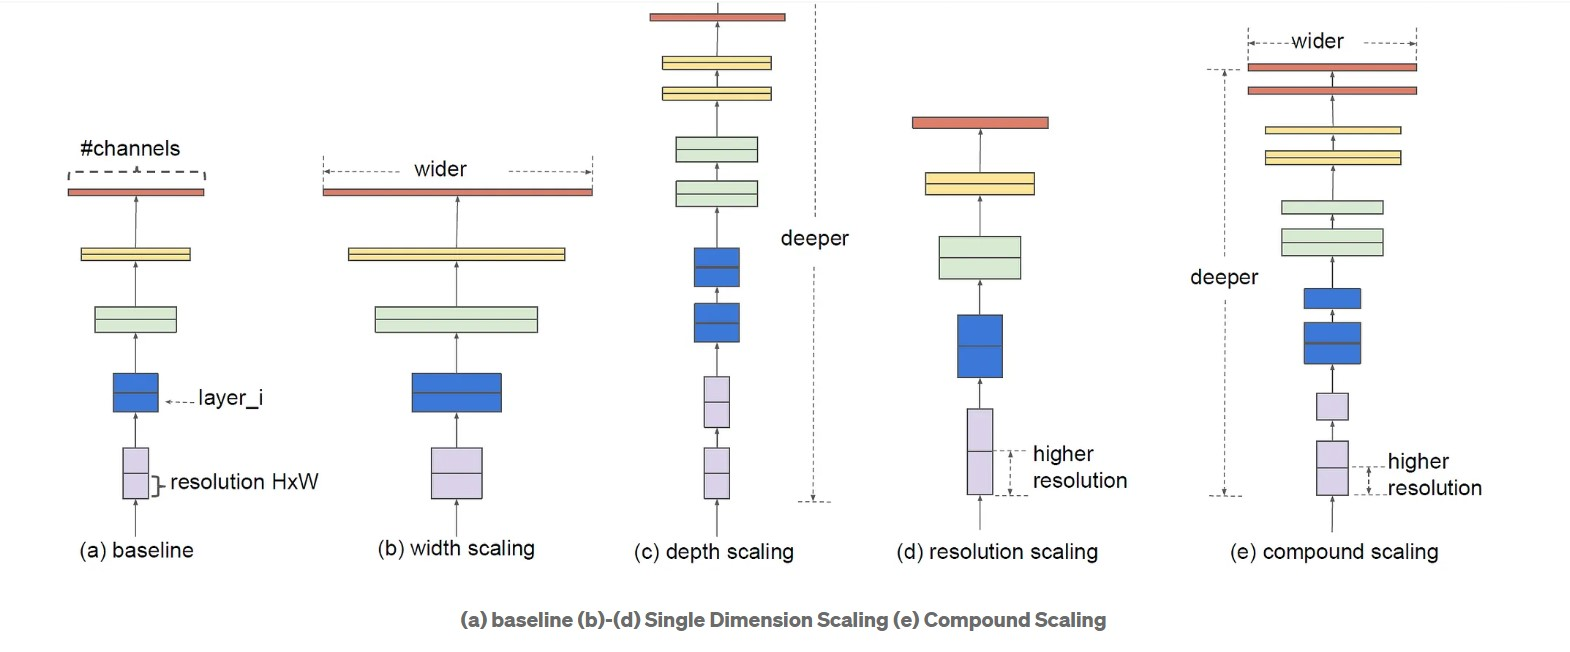
\includegraphics[height=6cm, width=9cm]{images/effwork.jpg}
    \caption{Figure 3 from Tan and Le (2020) illustrates the working of EfficientNetBO}
\end{figure}
\begin{enumerate}
  \item \textbf{Compound Scaling:} By uniformly scaling the model's width, depth, and resolution with a set ratio, this novel approach guarantees a balanced adjustment of these dimensions. With this approach, the model's performance is maximized without incurring exponentially higher computing costs\cite{tan2020efficientnet}.
  
  \item \textbf{Depthwise Separable Convolution:} EfficientNetB0 uses fewer computations and parameters than typical convolutional layers since it uses depthwise separable convolutional layers. This simplified architecture maintains representational capability while improving computing efficiency\cite{tan2020efficientnet}.
  
  \item \textbf{Inverted Residual Blocks:} EfficientNetB0 integrates inverted residual blocks with linear bottlenecks, drawing inspiration from MobileNetV2. These building components enable effective information transfer across the network, reducing computing burden and preserving high-quality feature representation\cite{tan2020efficientnet}.
  
  \item \textbf{Efficient Channel Attention (ECA):} By recalibrating channel-wise answers, ECA provides a lightweight technique for channel attention, improving feature representation. This addition increases the efficiency of the model by supporting its performance without dramatically increasing computational expenses\cite{tan2020efficientnet}.
  
  \item \textbf{Swish Activation Function:} Using this activation function, which has smoother behavior than more conventional activation functions like ReLU, allows EfficientNetB0 to operate more efficiently. This decision preserves computational economy while improving performance on a variety of jobs\cite{tan2020efficientnet}.
  
  \item \textbf{Model Scaling:} The compound coefficient ($\phi$) was introduced to allow for scalable model design. This means that practitioners can adjust the size of the model according to the computational resources that are available and the performance levels that they want\cite{tan2020efficientnet}.
\end{enumerate}


EfficientNet architecture consists of seven blocks which are shown in different colours. The basic building block of EfficientNet-B0 is a mobile inverted bottleneck convolution (MBConv), while each MBConv block is shown with the corresponding kernel filter size \cite{zhou2022multihead}. The figure below shows the different block:

\begin{figure}[!ht]
    \centering
    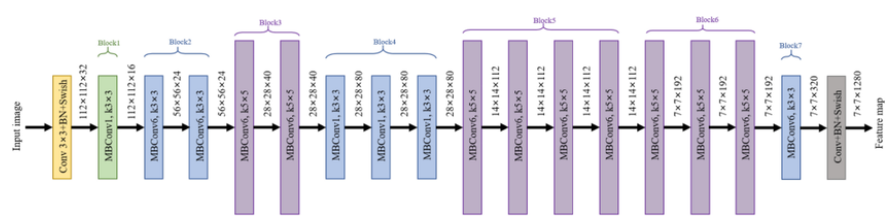
\includegraphics[height=6cm, width=9cm]{images/efflayer.PNG}
    \caption{Figure 3 from Zhou et al. (2022) illustrates the architecture of EfficientNetBO}
\end{figure}

The model comprises convolutional layers followed by depthwise separable convolutions. We modify this EfficientNetB0 by adding few layers and a classification layer. Global average pooling was used to reduce the parameter size. This layer not just reduce parameter also preserve the most important features by taking out the average. On top of that dense layer with ReLU activation was used further enhancing the model's ability to learn complex pattern in images, dropout regularization was used ensuring that the model could be generalized and does better on test set rather than just doing good only on training set. And a classification layer with sigmoid activation was used for binary classification. This architecture enables the development of a robust classification model capable of accurately distinguishing between edible and poisonous mushrooms.
//Anub
//Harith
//Harith
//Harith
//Harith
\appendix

\include{appendix01}



%%% APENDICES HERE

% \include{app11_research_paper_draft}

\let\section\chapter


\bibliographystyle{naturemag}

\bibliography{references}

% \renewcommand{\bibname}{Bibliography}

\end{document}
